% tesesusp.cls, v-0.0.1

% Based on 'bntex2ppgsi.cls', 'abntex2.csl' and on USP guidelines to create
% thesis and dissertation documents.
% See <https://www.overleaf.com/project/64f7bdf1641ad4a3a8482800>
% and <https://teses.usp.br/index.php?option=com_content&
%      view=article&id=52&Itemid=67&lang=en>
% to learn more.

\clearpage

% ----------------------------------------------------------------------
% Cover (mandatory)
% ----------------------------------------------------------------------

\imprimircapa

% ----------------------------------------------------------------------
% Title page (mandatory)
% ----------------------------------------------------------------------

%% Do not use this page for qualification exams.

\imprimirfolhaderosto*

% ----------------------------------------------------------------------
% Cataloging record (mandatory)
% ----------------------------------------------------------------------

%% Do not use for qualification exams.
\begin{fichacatalografica}
 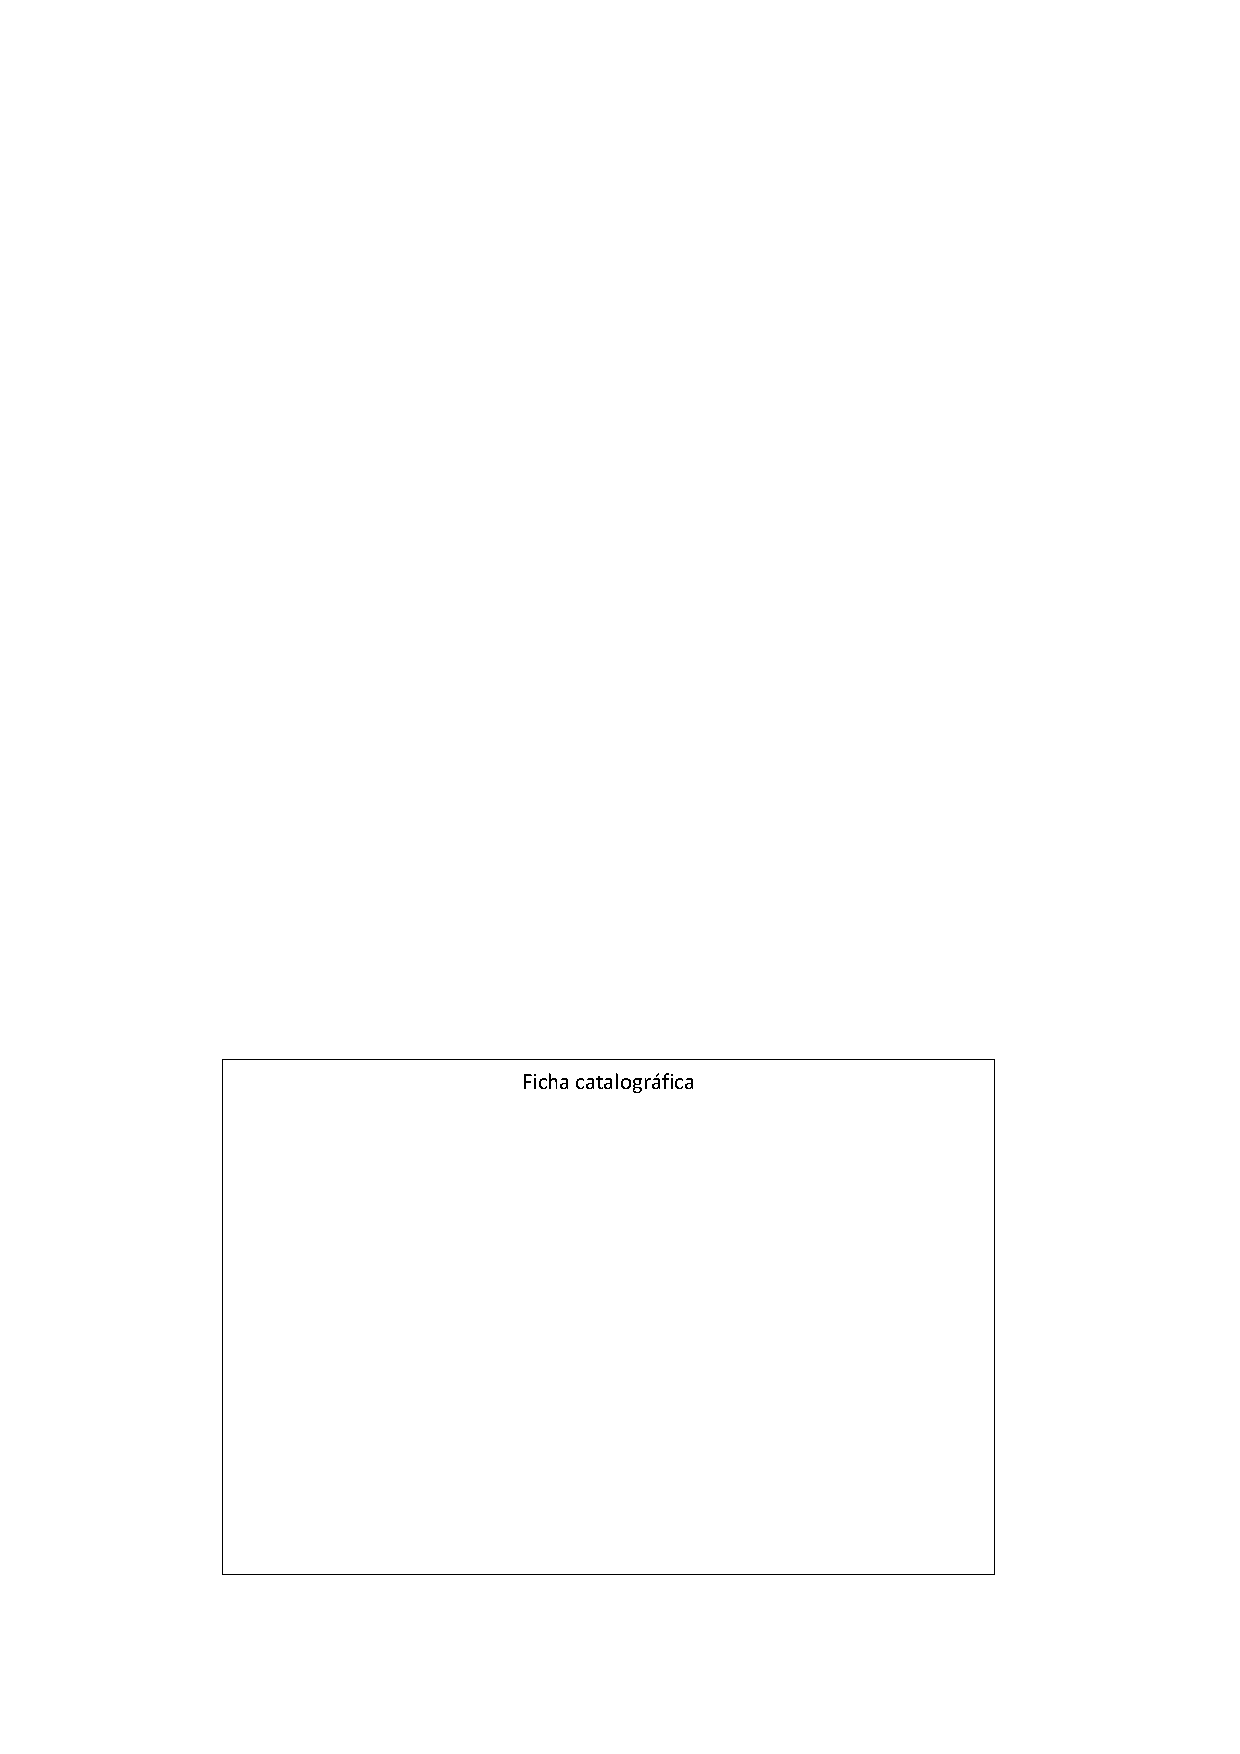
\includepdf{images/fig_ficha_catalografica.pdf}
\end{fichacatalografica}

% ----------------------------------------------------------------------
% Errata (optional)
% ----------------------------------------------------------------------

\begin{errata}
  \noindent
  This is the development version of the thesis (version <1.0.0). Any necessary corrections will be listed here after its approval.
\end{errata}

% ----------------------------------------------------------------------
% Approval sheet (mandatory)
% ----------------------------------------------------------------------

\begin{folhadeaprovacao}
\noindent
[TYPE OF EXAM] exam text by [AUTHOR'S FULL NAME], under the title \textbf{``\imprimirtitulo''}, presented to the [SCHOOL/DEPARTMENT] at the University of São Paulo, as part of the requirements for the degree of [TYPE OF DEGREE] by the [GRADUATE PRGRAM], in the concentration area of [CONCENTRATION AREA].

% [TYPE OF WORK] by [AUTHOR'S FULL NAME], under the title \textbf{``\imprimirtitulo''}, presented to the [SCHOOL/DEPARTMENT] at the University of São Paulo, as part of the requirements for the degree of [TYPE OF DEGREE] by the [GRADUATE PRGRAM]), in the concentration area of [CONCENTRATION AREA].

\vspace*{1.5cm}

\noindent
Approved on \_\_\_\_\_\_\_\_\_\_\_\_\_\_\_\_\_\_\_\_ , \_\_\_\_\_\_\_\_\_\_ .

\vspace*{1.5cm}

\begin{center}
\noindent Examination committee
\end{center}

\vspace*{0.5cm}

\noindent Committee chair:

\vspace*{0.25cm}

\renewcommand{\arraystretch}{2}
\setlength{\arrayrulewidth}{0pt}
\setlength{\tabcolsep}{0pt}
\noindent
\begin{tabular}{m{2cm} P{14cm}}
  Prof. Dr. & \_\_\_\_\_\_\_\_\_\_\_\_\_\_\_\_\_\_\_\_\_\_\_\_\_\_\_\_\_\_\_\_\_\_\_\_\_\_\_\_\_\_\_\_\_\_\_\_\_\_\_\_\_\_\_ \\
  Institution & \_\_\_\_\_\_\_\_\_\_\_\_\_\_\_\_\_\_\_\_\_\_\_\_\_\_\_\_\_\_\_\_\_\_\_\_\_\_\_\_\_\_\_\_\_\_\_\_\_\_\_\_\_\_\_ \\
\end{tabular}

\vspace*{1cm}

\noindent Examiners:

\vspace*{0.25cm}

\noindent
\begin{tabular}{m{2cm} P{14cm}}
  Prof. Dr. & \_\_\_\_\_\_\_\_\_\_\_\_\_\_\_\_\_\_\_\_\_\_\_\_\_\_\_\_\_\_\_\_\_\_\_\_\_\_\_\_\_\_\_\_\_\_\_\_\_\_\_\_\_\_\_ \\
  Institution & \_\_\_\_\_\_\_\_\_\_\_\_\_\_\_\_\_\_\_\_\_\_\_\_\_\_\_\_\_\_\_\_\_\_\_\_\_\_\_\_\_\_\_\_\_\_\_\_\_\_\_\_\_\_\_ \\
  Evaluation & \_\_\_\_\_\_\_\_\_\_\_\_\_\_\_\_\_\_\_\_\_\_\_\_\_\_\_\_\_\_\_\_\_\_\_\_\_\_\_\_\_\_\_\_\_\_\_\_\_\_\_\_\_\_\_ \\
\end{tabular}

\vspace*{0.5cm}

\noindent
\begin{tabular}{m{2cm} P{14cm}}
  Prof. Dr. & \_\_\_\_\_\_\_\_\_\_\_\_\_\_\_\_\_\_\_\_\_\_\_\_\_\_\_\_\_\_\_\_\_\_\_\_\_\_\_\_\_\_\_\_\_\_\_\_\_\_\_\_\_\_\_ \\
  Institution & \_\_\_\_\_\_\_\_\_\_\_\_\_\_\_\_\_\_\_\_\_\_\_\_\_\_\_\_\_\_\_\_\_\_\_\_\_\_\_\_\_\_\_\_\_\_\_\_\_\_\_\_\_\_\_ \\
  Evaluation & \_\_\_\_\_\_\_\_\_\_\_\_\_\_\_\_\_\_\_\_\_\_\_\_\_\_\_\_\_\_\_\_\_\_\_\_\_\_\_\_\_\_\_\_\_\_\_\_\_\_\_\_\_\_\_ \\
\end{tabular}

\vspace*{0.5cm}

\noindent
\begin{tabular}{m{2cm} P{14cm}}
  Prof. Dr. & \_\_\_\_\_\_\_\_\_\_\_\_\_\_\_\_\_\_\_\_\_\_\_\_\_\_\_\_\_\_\_\_\_\_\_\_\_\_\_\_\_\_\_\_\_\_\_\_\_\_\_\_\_\_\_ \\
  Institution & \_\_\_\_\_\_\_\_\_\_\_\_\_\_\_\_\_\_\_\_\_\_\_\_\_\_\_\_\_\_\_\_\_\_\_\_\_\_\_\_\_\_\_\_\_\_\_\_\_\_\_\_\_\_\_ \\
  Evaluation & \_\_\_\_\_\_\_\_\_\_\_\_\_\_\_\_\_\_\_\_\_\_\_\_\_\_\_\_\_\_\_\_\_\_\_\_\_\_\_\_\_\_\_\_\_\_\_\_\_\_\_\_\_\_\_ \\
\end{tabular}
\end{folhadeaprovacao}

% ----------------------------------------------------------------------
% Inscription (optional)
% ----------------------------------------------------------------------

\begin{dedicatoria}
  \vspace*{\fill}
  \centering
  \noindent
  \textit{
  Insert your dedication/inscription here.
  }
	\vspace*{\fill}
\end{dedicatoria}

% ----------------------------------------------------------------------
% Acknowledgments (optional)
% ----------------------------------------------------------------------

\begin{agradecimentos}
  \noindent
  I would like to acknowledge this awesome \href{https://github.com/danielvartan/tesesusp}{Quarto format}! :)
\end{agradecimentos}

% ----------------------------------------------------------------------
% Epigraph (optional)
% ----------------------------------------------------------------------

\begin{epigrafe}
  \vspace*{\fill}
	\begin{flushright}
	  \textit{Awesome quote} \\
		(Awesome quote citation)
	\end{flushright}
\end{epigrafe}

% ----------------------------------------------------------------------
% Abstract in the vernacular language (mandatory)
% ----------------------------------------------------------------------

\setlength{\absparsep}{18pt}
\begin{resumo}

\begin{flushleft}
[SURNAME], [INITIALS]. ([YEAR]). \textit{[TITLE]} [[TYPE OF THESIS]]. [SCHOOL/DEPARTMENT], University of São Paulo, São Paulo. [THESIS'S URL]
\end{flushleft}

Lorem ipsum dolor sit amet, consectetur adipiscing elit. Pellentesque accumsan rutrum lacus, vitae iaculis nisi bibendum in. Nulla et pellentesque nisl. Proin mollis dui sit amet egestas fermentum. Maecenas eu odio odio. Aenean porta ipsum in mauris pharetra dapibus. Nunc dapibus libero nec dui lacinia, id ultricies lectus maximus. Mauris quis mauris in velit pulvinar rutrum. Cras congue ante in orci luctus placerat. Nullam sit amet nisi augue. Maecenas non ligula eros. Etiam nec dolor a mi bibendum auctor.

Keywords: Keyword 1. Keyword 2. Keyword 3.
\end{resumo}

% ----------------------------------------------------------------------
% Abstract in the foreign language (mandatory)
% ----------------------------------------------------------------------

\begin{resumo}[RESUMO]
\begin{otherlanguage*}{brazil}

\begin{flushleft}
[SOBRENOME], [INICIAIS]. ([ANO]). \textit{[TÍTULO]} [[TIPO DE TESE/DISSERTAÇÃO]]. [ESCOLA/DEPARTAMENTO], Universidade de São Paulo, São Paulo. [URL DA DISSERTAÇÃO/TESE]
\end{flushleft}

Lorem ipsum dolor sit amet, consectetur adipiscing elit. Pellentesque accumsan rutrum lacus, vitae iaculis nisi bibendum in. Nulla et pellentesque nisl. Proin mollis dui sit amet egestas fermentum. Maecenas eu odio odio. Aenean porta ipsum in mauris pharetra dapibus. Nunc dapibus libero nec dui lacinia, id ultricies lectus maximus. Mauris quis mauris in velit pulvinar rutrum. Cras congue ante in orci luctus placerat. Nullam sit amet nisi augue. Maecenas non ligula eros. Etiam nec dolor a mi bibendum auctor.

Palavras-chaves: Palavra-chave 1. Palavra-chave 2. Palavra-chave 3.
\end{otherlanguage*}
\end{resumo}

% ----------------------------------------------------------------------
% List of figures (optional)
% ----------------------------------------------------------------------

\renewcommand{\listfigurename}{LIST OF FIGURES}
\pdfbookmark[0]{\listfigurename}{lof}
\listoffigures*
\cleardoublepage

% ----------------------------------------------------------------------
% List of tables (optional)
% ----------------------------------------------------------------------

\renewcommand{\listtablename}{LIST OF TABLES}
\pdfbookmark[0]{\listtablename}{lot}
\listoftables*
\cleardoublepage

% ----------------------------------------------------------------------
% List of abbreviations and acronyms (optional)
% ----------------------------------------------------------------------

\begin{siglas}
  \item[Abbreviation 1] Abbreviation expanded definition
  \item[Abbreviation 2] Abbreviation expanded definition
  \item[Abbreviation 3] Abbreviation expanded definition
\end{siglas}

% ----------------------------------------------------------------------
% List of symbols (optional)
% ----------------------------------------------------------------------

\begin{simbolos}
  \item[$\Gamma$] Gamma
  \item[$\Lambda$] Lambda
  \item[$\zeta$] zeta
\end{simbolos}

% ----------------------------------------------------------------------
% Table of contents (mandatory)
% ----------------------------------------------------------------------

\renewcommand{\contentsname}{TABLE OF CONTENTS}
\pdfbookmark[0]{\contentsname}{toc}
% \tableofcontents*
\cleardoublepage
